\documentclass[a4paper,10pt]{article}

\usepackage{amsmath}
\usepackage[utf8]{inputenc}
\usepackage{microtype}
\usepackage{hyperref}
\usepackage{tikz}

\begin{document}

\pagestyle{empty}
\noindent

\title{Udacity CarND Vehicle Detection and Tracking Project}
\author{Aleksander Czechowski}
\maketitle

The purpose of this project was to implement a vehicle detection and tracking algorithm.
The main goal of the project was to reliably detect the vehicles in the video project\_video.mp4.
The objective was achieved, as documented in the video output\_FINAL.mp4.
All the relevant code is contained in the notebook VD.ipynb.

\section{Rubric points}

\subsection{Histogram of oriented gradients}

\subsubsection{Explain how (and identify where in your code) you extracted HOG features from the training images. Explain how you settled on your final choice of HOG parameters.}

The features for the classifier were extracted by the \emph{extract\_features} function,
and were formed by a vector that consists of three parts:
%
\begin{itemize}
  \item spatial features,
  \item a color histogram,
  \item histogram of oriented gradients (\emph{hog}).
\end{itemize}

The code for each extraction is contained in functions 
\emph{bin\_spatial}, \emph{color\_hist}, and \emph{get\_hog\_features}, respectively.

Many adjustments have been made to find a combination of parameters that would give a satisfactory accuracy for the classifier.
As a rule of thumb, any combination that would yield accuracy below 99\% was discarded.
Once I found a combination, that gives accuracy of above 99\%, I decided to stick with it,
and try to improve the performance of the detector on the video during the video processing part.

After manual adjustment of 
I chose the following parameters for the histogram of gradients (the abbrieviations are the same as in the online course):

\begin{align*}
color\_space &= 'LUV' \\
orient &= 8 \\
pix\_per\_cell &= 8 \\
cell\_per\_block &= 2 \\
hog\_channel &= 0 \\
\end{align*}

The spatial binning features were set to $(32,32)$
and the number of color histogram feature bins was set to 32.

I was experimenting with $YCrCb$ color space that was reported to give good performance on the forums,
however I could not fine tune it to obtain satisfiable results.

\subsubsection{Describe how (and identify where in your code) you trained a classifier using your selected HOG features (and color features if you used them).}

The classifier was trained in the 5th block of code of the jupyter notebook,
the one starting with the comment \emph{HERE WE TRAIN THE CLASSIFIER}.

An instance of \emph{StandardScaler} was used to scale the features before training.
The same scaler was later used in the video pipeline in the \emph{find\_cars} function.

The classifier was trained by use of the Linear Support Vector Classification method with the default configuration.
The images, where a car is present were labelled with $1$, and the ones without a car with $0$.
The classifier based on Linear SVC method took about 13 seconds to complete the computations and achieved a test accuracy of 0.9903
(20\% of images were used to form the test set).


\subsection{Sliding window search}

\subsubsection{Describe how (and identify where in your code) you implemented a sliding window search. How did you decide what scales to search and how much to overlap windows?}

The sliding window implementation is contained in the function \emph{find\_cars},
which at the same time is used to make predictions.

One of the function arguments is \emph{scale}, which determines how to rescale 
the image accordingly to the size of vehicles expected to appear.
Images were divided into three (overlapping) parts, the first one represented where we expect the vehicles to be far from the camera,
the second -- where they are at medium distance, and the third -- where to look at close distance.
The remaining parts of the image are masked by adjusting the variables \emph{xstart, xstop, ystart, ystop} in each case.

The \emph{scale} factor was chosen by trial-and-error, the choice of $1.0$ for ``far'', $1.5$ for ``mid'' and $2.5$ for ``near'' worked quite well.
Each processed fragment image was divided into cells.
The hog features were extracted for all cells at once, and sub-sampled to obtain features for each window.
This greatly reduced the time of execution, as compared to separate sliding window implementation; the processing time on a modern laptop was similar to the length of the video,
which suggests that it could have been possible to implement the pipeline for real-time video processing.

The sliding windows were created by telling the function, how many cells to shift to obtain the next window (the variable \emph{cells\_per\_block}).
For this pipeline, I have chosen the same settings as in the classroom, since they gave reasonably good results.
The final settings were:
%
\begin{itemize}
  \item 8 pixels per cell,
  \item 8 cells per window (so 64 pixels in each window),
  \item 2 \emph{cells\_per\_block} (so 75\% overlap between the consecutive windows).
\end{itemize}

\subsubsection{Show some examples of test images to demonstrate how your pipeline is working. How did you optimize the performance of your classifier?}\label{subsection}

The pipeline is implemented in the \emph{process\_image} function.

As discussed in the previous subsection, the pipeline consists of three separate sliding window searches,
first one for far objects near the middle of the image, then for mid-ranged objects, a bit closer to the bottom,
and then for close objects, at the bottom of each image. This greatly enhances the chance of finding a vehicle,
regardless of its relative size in the camera snapshot.

To remove the duplicates and false positives, a heatmap approach ws used.
Based on the three searches, a heatmap was created. Wherever a detection occured,
a value of of $1$ was added to the heatmap, see function \emph{add\_heat}. 
Due to overlapping search windows, and overlapping search areas, 
the parts of the image containing a vehicle would obtain a high score.
Spurious detections, which result in a low score, were filtered by the function \emph{apply\_threshold},
which resets to $0$ all parts of a heatmap with score below a certain threshold.
The threshold was applied after each search (so separately for far/mid/near detection),
and the threshold values have been set (after some fine-tuning) to $2.1$/$1.0$/$1.5$, respectively.

At the end of each frame the heatmap was saved to variable \emph{saved\_heat}, and a fraction of it (with coefficient $0.92$, set by trial-and-error)
was added to the next heatmap. 
This represents the belief, that a vehicle on next frame is likely to appear close to the position of the vehicle on the previous frame, see Figure \ref{fig2}.
It also explains, why I have chosen fractional values for the thresholds.

\begin{figure}[h]
  \begin{center}
    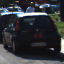
\includegraphics[width=50mm]{../snapshots/6.png}
    \quad
    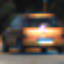
\includegraphics[width=50mm]{../snapshots/7.png}
\end{center}
\caption{The ``memory term'' allows to keep track of the vehicle even on a surface of similar color.}
\end{figure}\label{fig2}

The function \emph{scipy.ndimage.measurements.label} was applied to find the connected components of the filtered heatmap, see Figure \ref{fig1}.
Then, the function \emph{draw\_labeled\_bboxes} was used 
to draw bounding box at the positions of labeled areas on the original images.

\begin{figure}[h]
  \begin{center}
    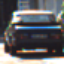
\includegraphics[width=50mm]{../snapshots/1.png}
    \quad
    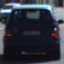
\includegraphics[width=50mm]{../snapshots/5.png}
\end{center}
\caption{The labeling-bounding box approach allows to merge duplicate detections.}
\end{figure}\label{fig1}

\subsection{Video Implementation}


\subsubsection{Provide a link to your final video output. Your pipeline should perform reasonably well on the entire project video 
(somewhat wobbly or unstable bounding boxes are ok as long as you are identifying the vehicles most of the time with minimal false positives.)}

The final video output can be found below:
\href{https://github.com/czechows/udacity----vehicle-detection/blob/master/output_FINAL.mp4}{https://github.com/czechows/udacity----vehicle-detection/blob/master/output\_FINAL.mp4}.

As one can see, both the white and the black vehicle are tracked throughout the whole video, though the size and shape of the bounding box evolves.
There are almost no multiple detections for single vehicles, and if a multiple detection forms,
it is quickly merged into a single detection (e.g. Figure \ref{fig1}).


\subsubsection{Describe how (and identify where in your code) you implemented some kind of filter for false positives and some method for combining overlapping bounding boxes.}

The filter for false positives is implemented in the \emph{apply\_threshold} function,
and the overlapping bounding boxes are combined by the \emph{scipy.ndimage.measurements.label} function,
which identifies connected components of the positive part of the heatmap.
A ``memory'' term was added to the heatmap to increase the probability of finding vehicles near the detections from previous frames.

The precise explanation is included in the answer to the rubric point \ref{subsection}, where I describe my pipeline, and show images which relate to the question.

\subsection{Discussion}

\subsubsection{Briefly discuss any problems / issues you faced in your implementation of this project. Where will your pipeline likely fail? What could you do to make it more robust?}

In the choice of parameters, I took a conservative approach, that it is better to detect too much than too little.
In real world this would be crucial for the safety of the autonomous vehicle.

Such goal forced me to choose a fairly high value of the ``memory'' term,
so I could track both vehicles throughout the whole video, without losing them at any of the frames.
The downside of the approach is that there are still some false positives in the video,
although they disappear fairly quickly, as the video progresses (see Figure \ref{fig3}).

A larger dataset and a better classifier (perhaps a neural network) would allow to reliably detect e.g. white vehicles on white background, 
remove the need for the memory term, and reduce the number of false positives.

\begin{figure}[h]
  \begin{center}
    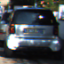
\includegraphics[width=60mm]{../snapshots/4.png}
\end{center}
\end{figure}\label{fig3}

\end{document}

